\FloatBarrier

\section{Softwarebasierte Digitalisierung von historischen Toninformationsträgern}

\subsection{Das \code{musicbox} Paket}

\begin{figure*}[t]
    \centering
    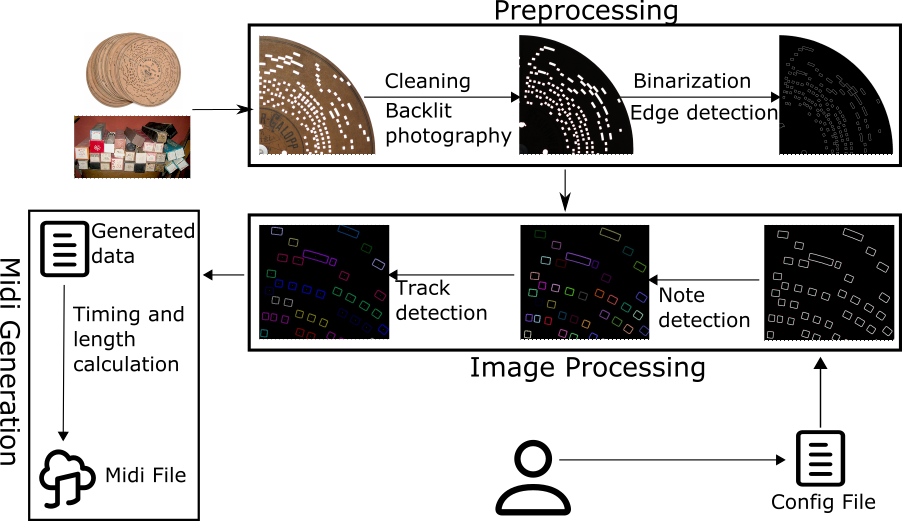
\includegraphics[width=\textwidth]{graphics/flow_diagram.png}
    \caption{Übersicht über den Digitalisierungsprozess einer Lochplatte mit der \code{musicbox} Software.}
    \label{softwareworkflow}
\end{figure*}

Im Rahmen des DISKOS-Projektes soll eine einheitliche Softwarelösung für die Generierung von Midi-Dateien aus Bildern der Toninformationsträger im Bestand des Musikinstrumentenmuseums der Universität Leipzig erstellt werden.
Zu diesem Zweck wurde die, dieser Arbeit zugrundeliegende, Software in Form des \code{musicbox} Paketes in der Programmiersprache Python \parencite[]{van1995python} implementiert.
Diese Software ermöglicht es den gesamten Umwandlungsprozess von der Vorverarbeitung der Bilddaten bis zur Erstellung der Midi-Datei automatisiert vorzunehmen.
Es werden während der Verarbeitung idealerweise keine externen Eingaben benötigt.

Um die für die Verarbeitung der diversen unterschiedlichen Formate von Toninformationsträgern notwendige Flexibilität zu ermöglichen und gleichzeitig eine möglichst hohe Wiederverwendbarkeit der einzelnen Bestandteile zu gewährleisten, ist die Software modular aufgebaut und durch Konfigurationsdateien flexibel anpassbar.
Mit diesem Ansatz soll in der Zukunft für die Verarbeitung eines neuen Formats von Toninformationsträgern idealerweise die Erstellung einer Pipeline aus einzelnen Verarbeitungsschritten und die Angabe von Formatspezifischen Informationen wie Spurenbelegung, Abmessungen etc. ausreichen.

Diese Funktionalität wird über Profile, die in einer YAML-Konfigurationsdatei hinterlegt sind, realisiert.
In dieser wird für ein Profil zunächst eine Pipeline bestehend aus mehreren Verarbeitungsschritten definiert.
Die verfügbaren Verarbeitungsschritte sind innerhalb des Paketes in mehreren Python-Dateien nach dem Teilgebiet des Umwandlungsprozesses zu dem sie gehören aufgeteilt.
Der Name des Verarbeitungsschrittes setzt sich dabei aus Datei und Methodennamen zusammen, z.B. \code{preprocessing.binarization}.
Neben der Verarbeitungspipeline werden die für den Umwandlungsprozess benötigten Parameter in der Konfigurationsdatei abgelegt.
Diese beinhalten Metadaten zum Format des Mediums das verarbeitet werden soll, etwa die Anzahl und die Belegung der vorhandenen Spuren, aber auch Parameter für die Vorverarbeitung der Bilddaten, etwa den Threshold für die Bildbinarisierung.

Die Software ist dabei auf einfache Erweiterbarkeit ausgelegt.
Neue Verarbeitungsschritte können als Methode in der entsprechenden Python-Datei definiert werden und werden dann, wenn sie Bestandteil einer Verarbeitungspipeline sind, automatisch zur Laufzeit aufgerufen.
Zusätzlich können in einer separaten Konfigurationsdatei Metainformationen zum Verarbeitungsschritt definiert werden.
In dieser Datei werden Informationen zu den für den Verarbeitungsschritt erforderlichen Parametern, sowie aus anderen Verarbeitungsschritten benötigten bzw. für diese bereitgestellten Daten gespeichert.
Diese Informationen nutzt die Software, um vor der Ausführung einer Verarbeitungspipeline zu prüfen, ob diese ausführbar ist und ob alle benötigten Parameter im Konfigurationsprofil definiert sind.

Der Umwandlungsprozess selbst kann entweder über das Einbinden des Paketes in ein eigenes Python-Skript oder über ein bereitgestelltes Wrapper-Skript angestoßen werden.
In Abbildung \ref*{softwareworkflow} ist eine grobe Übersicht über den allgemeinen Umwandlungsprozess zu sehen.

Grundlegend gilt es im Umwandlungsprozess von Lochplatten und Notenrollen die Informationen über Tonhöhe, -anfang und -länge zu finden.
Dazu müssen zunächst die einzelnen Löcher auf dem Medium identifizieren werden.
Für jedes dieser Löcher sind im Folgenden der Start- und Endpunkt der Lochung auf dem Medium zu identifiziert, aus welchen Tonanfang und -länge abzuleiten sind.
Abschließend muss jedes Loch noch der entsprechenden Spur auf dem Medium zugeordnet werden, um die Tonhöhe bestimmen zu können.

Ziel der Umwandlung ist in jedem Fall die Erstellung einer Midi-Datei.
Eine solche speichert keine Audioinformationen, sondern, nicht unähnlich der ursprünglichen Toninformationsträger, Informationen wann welcher Ton für wie lange klingt.
Midi-Dateien können als etablierter Standard für die Speicherung solcher Informationen betrachtet werden und sind das Umwandlungsziel oder -zwischenziel bei allen aktuelleren Verfahren zum Digitalisieren von Toninformationsträgern, siehe etwa \textcite[65]{colmenares_2011} oder \textcite[518]{shi_2019}.

Im Folgenden wird dieser Umwandlungsprozess anhand einer voll funktionalen Pipeline für die Umwandlung von Lochplatten, sowie einer sich noch im Prototypstadium befindlichen Pipeline für Notenrollen genauer erläutert.

\subsection{Digitalisierung von Pappplatten}

\begin{figure*}[t]
    \centering
    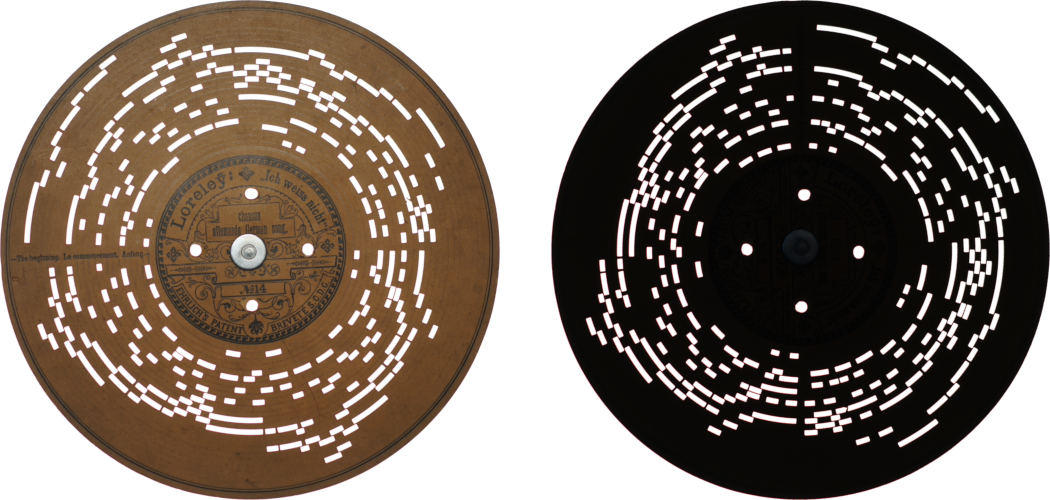
\includegraphics[width=\textwidth]{graphics/ariston_pictures.png}
    \caption{Zur Dokumentation angefertigtes Bild einer Lochplatte sowie das für die Digitalisierung bestimmte Bild der gleichen Lochplatte.}
    \label{pappplattenphotos}
\end{figure*}

Lochplatten sind die ältesten Toninformationsträger, die im Rahmen des DISKOS-Projekts digitalisiert werden sollen.
Die Verarbeitung der Lochplatten ist durch die runde Form etwas komplexer als die von Notenrollen.
Gleichzeitig sind die auf den Medien kodierten Toninformationen vergleichsweise simpel, es sind keine Steuerungsinformationen oder ähnliches vorhanden.
Auch reduziert die relativ kleine Größe der Medien die rechnerische Komplexität des Unwandlungsprozesses im Vergleich zu Notenrollen.\footnote{Vorliegende Notenrollenscans erreichen bei 300 DPI Dateigrößen bis zu 5GB.}
Sie wurden deshalb als erstes Format für die Umwandlung in Midi-Dateien ausgewählt.

Der Digitalisierungsprozess beginnt mit der Begutachtung der Medien durch am Projekt beteiligte Musikwissenschaftler:innen, die die Medien reinigen, auf Schäden untersuchen und anschließend alle auf dem Medium selbst vorhandenen Metainformationen, zusammen mit allen gefundenen Beschädigungen des Mediums, dokumentieren.
Anschließend wird eine hochauflösende Fotografie des Mediums angefertigt.
Die Lochplatten werden dazu in einer, speziell für diesen Zweck konstruierten, Aufhängung platziert, in welcher sie mit Hintergrundbeleuchtung fotografiert werden können.
Abbildung \ref{pappplattenphotos} zeigt beispielhaft das Bild einer Lochplatte der Marke Ariston, sowohl als normales Foto als auch als Bild für die weitere digitale Verarbeitung.

Die Bilder, die für die softwarebasierte Verarbeitung vorgesehen sind, unterscheiden sich dabei von denen, die zur Dokumentation und Konservierung angefertigt werden.
Während die Platten für die normalen Fotografien nach der Plattenbeschriftung ausgerichtet werden, werden die Lochplatten für die weitere Digitalisierung mit der Startmarkierung der Lochplatte auf 0 Grad ausgerichtet.
Dadurch entfällt die Notwendigkeit die Startmarkierung softwareseitig zu identifizieren.
Auch werden diese Aufnahmen mit veränderten Belichtungseinstellungen vorgenommen, um einen höheren Kontrast zwischen den Löchern auf der Platte und der Platte selbst zu erreichen.\footnote{Während der anfänglichen Entwicklung der hier vorgestellten Software wurden für die Verarbeitung Bilder ohne diese Einstellungen oder Hintergrundbeleuchtung erfolgreich verwendet. Es ist davon auszugehen, dass sich solche Bilder mit leichten Anpassungen der Vorverarbeitung problemlos verwenden lassen.}

Die vorliegenden Bilddaten werden für die weitere Verarbeitung grundsätzlich als Graustufenbild eingelesen.
Im Anschluss wird zunächst eine einfache, threshold-basierte Binarisierung angewendet.
Für diesen, sowie die meisten weiteren bildbasierten Verarbeitungsschritte, wird die OpenCV \parencite[]{opencv_library} Bibliothek im Zusammenspiel mit Numpy \parencite[]{harris2020array} genutzt.
Der genutzte untere Threshold für die Binarisierung (60) wurde experimentell ermittelt, um eine möglichst optimale Erhaltung der Strukturen der Platten, bei gleichzeitiger Minimierung von Artefakten zu gewährleisten.

Im nächsten Schritt wird ein Kantenerkennungsalgorithmus auf das Bild angewendet.
In früheren Versionen der Software wurde hierfür der Canny-Algorithmus eingesetzt \parencite[]{canny_1986}.
Dies führte mitunter zu Problemen, da die Abstände zwischen einzelnen Löchern auf den Pappplatten in Extremfällen nur einzelne Pixel betragen und die mit dem Canny-Algorithmus berechneten Kanten sich in solchen Fällen überlappen können.
Um dieses Problem zu umgehen wird ein morphologischer Kantenerkennungsalgorithmus eingesetzt, der zunächst mit einem 3x3 Kernel eine Erosion des Bildes durchführt und anschließend aus der Differenz des Originalbildes und der Erosion die Kanten bildet.
Dieses Verfahren stellt sicher, dass die Kanten immer auf der Innenseite der Löcher der Lochplatten liegen.

\begin{figure*}[t]
    \centering
    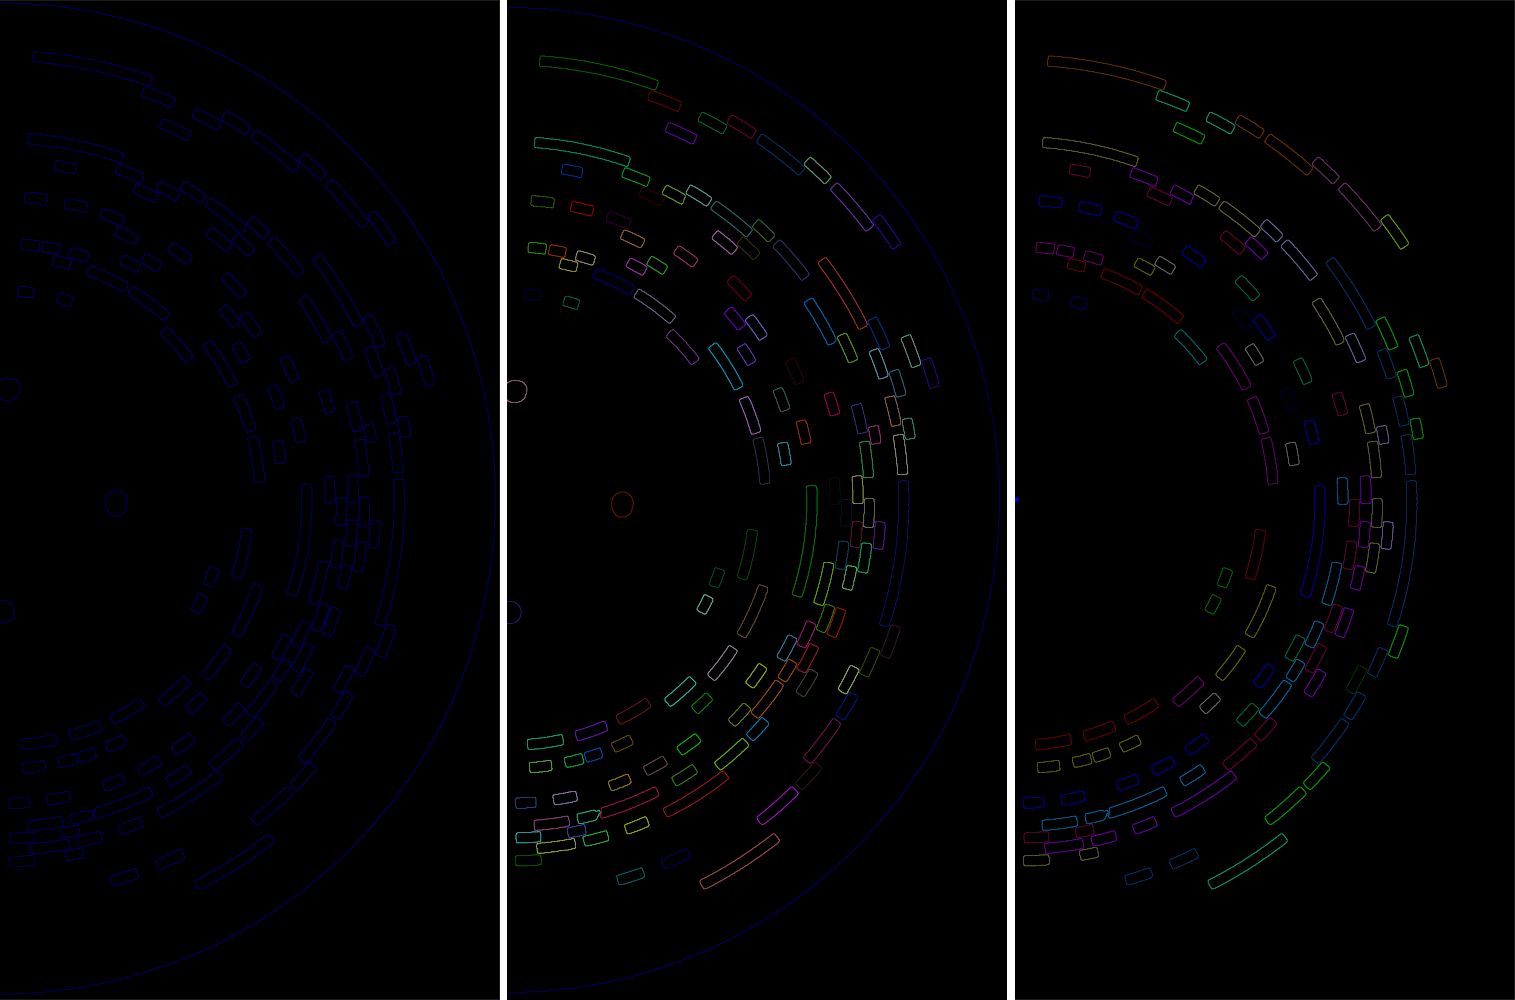
\includegraphics[width=\textwidth]{graphics/processing.png}
    \caption{Bild einer Ariston Lochplatte nach der Kantenerkennung, dem Identifizieren von Löchern sowie der Zuordnung der Löcher zu Spuren.}
    \label{pipelinesteps}
\end{figure*}

Um das nun vorliegende Bild der Kanten weiter zu Zerlegen und Komponenten wie die einzelnen Notenlöcher identifizieren zu können, wird im weiteren ein Algorithmus zum Finden von 2-verbundenen Komponenten aus Scikit-Image \parencite[]{scikit-image} eingesetzt.
Die so gefundenen Komponenten werden für die weitere Verarbeitung in jeweils ein Array mit den Koordinaten der zugehörigen Pixel umgewandelt, um Berechnungen von Distanzen etc. zu vereinfachen.
Aus diesen Komponenten wird die äußere Kante der Platte identifiziert (die größte zusammenhängende Komponente), sowie rechnerisch, mithilfe von in der Konfiguration hinterlegten Messungen, die innere Grenze des mit Tonspuren belegten Bereichs bestimmt.
Es werden alle gefundenen Komponenten die innerhalb dieser inneren Begrenzung oder außerhalb des äußeren Plattenrandes liegen herausgefiltert, da diese keine Tonlöcher sein können und somit für die weitere Verarbeitung uninteressant sind.

Alle verbleibenden Komponenten sind die Kanten von Löchern auf der Lochplatte.
Einzelne Platten weisen Beschädigungen in der Form von Einrissen zwischen zwei Löchern auf, die dazu führen können, dass diese Löcher als eine gemeinsame Komponente und damit im Weiteren als ein Einzelner, über die gesamte Länge der beiden Löcher klingender, Ton interpretiert werden.
Dies entspricht allerdings auch dem Verhalten eines Originalabspielgerät beim Abspielen einer Platte mit solchen Beschädigungen, so sie denn in einem insgesamt noch spielbereiten Zustand ist.
Um zu gewährleisten, dass das Digitalisat dem tatsächlich vorliegenden Medium so ähnlich wie möglich ist, findet deshalb keine Korrektur solcher Einrisse statt.

Im nächsten Schritt wird der Mittelpunkt der Lochplatte bestimmt.
Da die Lochplatten beim Fotografieren an dem Loch in ihrer Mitte aufgehängt werden, ist dieses auf den Bildern nicht identifizierbar.
Zur Mittelpunkbestimmung wird deshalb ein rechnerisches Verfahren angewendet.
Es wird mittels des Algorithmus von \textcite[]{halir1998numerically} eine Ellipse auf die Punkte des äußeren Plattenrandes regressiert und anschließend aus der Ellipsengleichung der Mittelpunkt bestimmt.
Dieses Verfahren liefert grundsätzlich sehr akkurate Ergebnisse, hat jedoch bei einzelnen Lochplatten mit bestimmten Deformationen Probleme.
Dort wird zwar der korrekte Mittelpunkt des äußeren Plattenrandes identifiziert, dieser ist aber nicht der Mittelpunkt der Tonspuren auf der Platte.
In diesen Fällen ist aktuell eine manuelle Korrektur des Mittelpunkts nötig.

Anschließend werden die einzelnen erkannten Löcher ihren entsprechenden Spuren zugeordnet, so dass die jeweiligen Tonhöhen bestimmt werden können.
Dafür wird zunächst die Distanz, vom Zentroid ausgehend, jeder Komponente zum äußeren Rand sowie zum Mittelpunkt der Lochplatte berechnet.
Aus diesen Distanzen wird die relative Position der Komponente zwischen dem Plattenmittelpunk und dem Plattenrand abgeleitet.
Dies dient zur Reduzierung des Einflusses von Deformationen der Lochplatte auf den Spurzuordnungsprozess.
Anhand dieser Positionen werden die Komponenten in die einzelnen Spuren gruppiert, wozu das MeanShift Clusteringverfahren \parencite[]{meanshift} in der Implementierung in Scikit-Learn \parencite[]{scikit-learn} eingesetzt wird.
Dieses Verfahren wurde gewählt, da es gegenüber den meisten Algorithmen, die spezifisch für das Gruppieren von eindimensionalen Daten entwickelt wurde, den Vorteil bietet kein a priori Wissen über die Anzahl der Cluster zu benötigen.
Da nicht notwendigerweise alle Spuren, die ein Format bietet bei jeder Platte des Formats genutzt werden, ist nur die obere Schranke der Zahl der Cluster bekannt, nicht aber die Zahl der tatsächlich vorhandenen.

Dies beeinflusst auch die Zuordnung der in dem Format existierenden Spuren, zu denen auf dem spezifischen Medium gefundenen.
Um für das Vorhandensein leerer Spuren zwischen den gefundenen Spuren zu kompensieren, wird die durchschnittliche Distanz der gefundenen Spuren zu den jeweiligen Nachbarn berechnet und jeweils zwischen die Spuren mit der höchsten Distanz eine leere Spur eingefügt.
Dies wird wiederholt, bis die Zahl der vorhandenen Spuren der der in dem Format existierenden Spuren entspricht.
Ist dieser Schritt abgeschlossen sind die gefundenen Löcher ihren Spuren zugeordnet und die mit ihnen verbundene Tonhöhe ist ermittelt.

Um die nun noch fehlenden Informationen zu Tonanfang und -länge zu finden, wird für jedes Loch das minimal umschließende Rechteck berechnet.
Anhand dessen wird je ein Punkt am, im Sinne der Abspielrichtung der Lochplatte, Anfang und Ende des Lochs bestimmt.
Für beide Punkte wird dann, ausgehend vom Plattenmittelpunkt, der Winkel zwischen Punkt und dem Rollenanfang berechnet.
Der kleinere Winkel ist der Tonanfang, der Zeitpunkt an dem die Note zu klingen beginnt, die Differenz der beiden Winkel die Tonlänge, die Zeit für die der Ton klingt.

Die Originalabspielgeräte für diese Medien spielen Töne leicht verzögert zum Erreichen des Loches ab.
Dies ist in der Bauweise begründet, erst wenn eine bestimmte Menge Luft durch ein Ventil strömt entsteht ein hörbarer Ton, üblicherweise wenn etwa die Hälfte eines Ventils frei liegt.
Ein ähnliches Verhalten ist auch beim Schließen der Ventile am Lochende zu beobachten.
Aktuell findet hierfür keine Anpassung statt, dies wäre aber in der Zukunft über Konfigurationsparameter vorstellbar.

Weiterhin ist anzumerken, dass die berechneten Angaben zu Timing und Tonlänge in Grad vorliegen und nicht in Schlägen, wie sie in Midi-Dateien kodiert sind.
Während softwareseitig Methoden bereitgestellt werden um diese Angaben um einen festen Faktor zu skalieren, ist eine genaue Bestimmung des Zeitmaßes nicht zuletzt dadurch erschwert, dass es sich bei den Originalabspielgeräten um handbetriebene Automaten handelte.
Das Tempo war deshalb abhängig von der Drehgeschwindigkeit der Kurbel und somit variabel.
Eine bessere Bestimmung des Zeitmaßes würde vermutlich durch die Bestimmung von Takt- und Schlaglänge des Stückes auf dem Medium möglich, die aber nicht zum aktuellen Funktionsumfang der Software gehört.

Aus den bis hier gewonnen Informationen wird abschließend mittels der MIDIUtil Bibliothek \parencite[]{midiutil} eine Midi-Datei erstellt, die die auf dem Toninformationsträger kodierten Informationen enthält.
Diese Dateien können anschließend beliebig weiterverwendet werden.
Eine Überführung in eine Auralisierung, in Form einer Audiodatei, kann entweder über generische Softwareinstrumente erfolgen oder z.B. über die, sich ebenfalls am Musikinstrumentenmuseum in Entwicklung befindliche, midiAuralizer \parencite[]{midiauralizer} Software.
Diese ermöglicht es beliebige Midi-Dateien mittels, im Rahmen des DISKOS-Projekts aufgenommener, Tonvorräte von historischen Instrumenten, darunter auch Originalabspielgeräte für Lochplatten des Typs Ariston, zu Audiodateien umzuwandeln.

Das hier vorgestellte Verfahren wurde in dieser Form für die Umwandlung des gesamten Konvolutes der Lochplatten des Types Ariston verwendet.
Ebenso konnte es in testweisen Digitalisierungsversuchen mit Lochplatten für einen mechanischen Klaviervorsteller ähnlich gute Ergebnisse erzeugen.
Die nötigen Anpassungen beschränken sich dabei auf die Erstellung eines neuen Konfigurationspresets mit Informationen zu den Abmessungen und Spuren des neuen Formats.

\subsection{Digitalisierung von Klavierrollen}

Als nächster Schritt der Entwicklung der vorgestellten Softwarelösung wurde ein vergleichsweise simples Format von Notenrollen für die Digitalisierung ausgewählt, Notenrollen der Marke Hupfeld Phonola Solodant.
Notenrollen dieses Formats besitzen 77 Spuren, von denen 73 Spuren Tönen zugeordnet sind, 2 zur Dynamiksteuerung verwendet werden und 2 freibleiben.

Während das vorgestellte Digitalisierungsverfahren für Lochplatten als voll funktionsfähig angesehen werden kann, befindet sich die Lösung für die Umwandlung von Notenrollen noch in einem früheren Entwicklungsstadium und sollte als Prototyp verstanden werden.
So werden die auf den Rollen vorhandenen Steuerspuren zwar korrekt ausgelesen, aber bei der Generierung der MIDI-Dateien aktuell nicht genutzt.
Auch können, zum Teil auf den Rollen abgedruckte, Dynamiklinien durch das Verfahren aktuell nicht ausgewertet werden.
Dennoch stellt das Verfahren in seinem aktuellen Zustand eine grundlegend funktionsfähige Digitalisierunglösung für Notenrollen dar.
Auch zeigt sich im Hinblick auf die Umsetzung des Verfahrens der Vorteil einer modularen Softwarelösung wie der hier vorliegenden.
Während viele Komponenten speziell für die Verarbeitung von Notenrollen implementiert wurden, konnte ein Teil der Komponenten aus dem bereits vorgestellten Prozess wiederverwendet werden.

Die, währen des vorangegangenen TASTEN-Projekts in Zusammenarbeit mit einem externen Dienstleister erstellten, vollständigen Scans von Notenrollen liegen als TIFF-Dateien mit einer Auflösung von 300 DPI vor und bilden die gesamte Notenrolle inklusive Anfang und Ende ab.
Diese Scans wurden, im Gegensatz zu den im Rahmen des DISKOS-Projektes erzeugten Aufnahmen von Lochplatten, vor schwarzem Hintergrund ohne Hintergrundbeleuchtung erstellt.
Aus technischen Gründen umfassen die Scans, je nach Rollenlänge, auch einen längeren, leeren Bereich nach dem Ende der Rolle.

Nach der Binarisierung der Bilder, die mit der gleichen Komponente wie die der Lochplatten erfolgt, wird daher zunächst die Rolle auf die Länge des tatsächlich gelochten Teils gekürzt.
Um diesen Bereich zu identifizieren, wird über die gesamte Länge des Scans für jede Zeile der relative Anteil der Pixel mit Inhalt errechnet.
Anschließend wird bestimmt in welchen Zeilen der Anteil der gefüllten Pixel über 80\% liegt\footnote{Die Scans der Notenrollen weisen einen, je nach Format, unterschiedlich großen Rand neben der Rolle auf. 80\% wurde experimentell als sinnvolle untere Schranke bestimmt.} und aus diesen die längste zusammenhängende Folge von Zeilen ausgewählt.
Diese Methode schließt, je nach konkret betrachtetem Scan, einen gewissen Teil von Rollenanfang und -ende mit ein, dies erwies sich jedoch in der Praxis als unproblematisch für die weitere Verarbeitung.

Die folgenden Schritte des Findens von zusammenhängenden Komponenten sowie das Umwandeln dieser in Koordinatenlisten geschehen mit den gleichen Verfahren, die auch für Lochplatten genutzt wurden.
Um die Ränder der Rolle zu identifizieren, werden über die gesamte Länge der Rolle 100 zufällige Zeilen ausgewählt und die in diesen Zeilen liegenden verbundenen Komponenten gezählt.
Die beiden Komponenten die in den meisten, praktisch sogar allen, Zeilen vorkommen sind die Kanten an den Rändern der Rolle.

Aufgrund der unterschiedlichen Aufnahmetechnik der Notenrollen, gegenüber den später aufgenommenen Platten, weisen sie nach der Binarisierung und Kantenerkennung deutlich mehr Artefakte auf.
Um dies zu kompensieren, werden im nächsten Schritt Filter auf die gefundenen Komponenten angewendet.
Zum einen wird für jede verbundene Komponente ermittelt, ob sie aus mehr oder weniger Pixeln besteht als der über die Pixelzahl aller verbundenen Komponenten, mit Ausnahme der Rollenränder, gebildete Mittelwert.
Alle Komponenten, die aus weniger Pixeln bestehen als die durchschnittliche Komponente werden entfernt.
Die verbleibenden Komponenten werden noch einmal über ihre Form gefiltert.
Es wird geprüft ob das gerundete Verhältnis von Höhe zu Breite der Komponente im Intervall $[1,2]$ liegt.
Während ein rundes Loch in einer Notenrolle üblicherweise etwa genau so breit wie hoch sein sollte, kann es bei sehr eng platzierten Löchern dazu kommen, dass diese als eine gemeinsame Komponente erkannt werden.
Deshalb werden solche Komponenten, die bis etwa doppelt so hoch wie breit sind, nicht entfernt.
Abgesehen von einzelnen Verarbeitungsfehlern sind alle noch verbleibenden Komponenten die Kanten von Löchern auf der Notenrolle.

Anschließend werden die Informationen zu den auf der Rolle kodierten Noten extrahiert.
Zu diesem Zweck wurde im Rahmen des DISKOS-Projekts von Musikwissenschaftler:innen der Gleitbock des Abspielgerätes\footnote{Die Komponente auf der die Notenrolle aufliegt und an der das Vakuum anliegt das für die Tonerzeugung nötig ist.} vermessen und die genauen Maße, sowie der assoziierte Ton für jede Spur dokumentiert, siehe \textcite[]{mxp_2002548}.
Mit diesen Informationen kann, durch einfaches Berechnen der relativen Distanzen zwischen jedem Loch und den Rollenrändern, die zugehörige Spur für jedes Loch ermittelt werden.
Da Notenrollen sich, bedingt durch die lange Zeit der Lagerung, insbesondere im späteren Verlauf der Rolle verziehen können, wird die Rolle für diese Berechnungen in Segmente zu jeweils mindestens 1000 Pixeln unterteilt und die Positionsbestimmung für jedes Segment separat vorgenommen.
Die Segmente werden dabei so gewählt, dass kein Loch geteilt wird.
Sollte der Bedarf bestehen können diese Segmente auch kleiner gewählt werden, die gewählte Größe hat sich jedoch bis jetzt als ausreichend erwiesen, um, zumindest leichte, Deformationen der Rolle ausgleichen zu können.
Gleichzeitig sollte diese Größe noch ausreichend groß sein, um zu verhindern, dass kürze Einriss der Rolle oder ähnliche Beschädigungen die Spurbestimmung negativ beeinflussen.
Tonanfang und -länger werden durch die Position des höchsten und tiefsten Punkts einer Komponente bestimmt.

Im Gegensatz zu den Abspielgeräten für Lochplatten wurden Reproduktionsklaviere meist von elektrischen Motoren betrieben und erlaubten so eine präzise Einstellung der Abspielgeschwindigkeit.
Die vorgesehene Abspielgeschwindigkeit war bei einigen Formaten auf dem Rollenanfang, in der Einheit feet per 10 Minutes vermerkt \parencite[63]{colmenares_2011}.
Da die Scanauflösung bekannt ist, kann der Umrechnungsfaktor Pixel per Second ($pps$) aus den feet per minute ($fpm$) wie in Gleichung \ref{eq:1} errechnet werden.
Werden die vorher ermittelten Timings und Tonlängen nun mit diesem Faktor skaliert, liegen die Tonlängen in Sekunden vor.
Zeitangaben in MIDI-Dateien erfolgen grundsätzlich als Schläge (Beats) und nicht in Sekunden, \footnote{Alternativ ist es auch möglich die Zeitangaben in Ticks zu hinterlegen, diese stehen allerdings in einem direkten Verhältnis zu Schlägen.} weshalb zusätzlich die Geschwindigkeit der erzeugten Midi-Datei auf 60 BPM festgelegt wird.
Mittels dieser Skalierung sollten die Digitalisate der Notenrollen mit vorhandenen Tempoangaben annähernd im Originaltempo abgespielt werden.

\begin{equation} \label{eq:1}
    pps = \frac{fpm * 12 * 300}{60}
\end{equation}

Aufgrund der mechanischen Eigenschaften der Pneumatik der Originalabspielgeräte wurden Löcher, die einen sehr kleinen Abstand zueinander hatten wie ein durchgehendes Loch abgespielt.
Die praktische Grenze dieses Verhaltens ist nicht klar bekannt und dürfte zwischen Geräten variieren.
\textcite[7]{zoltan_1994} gibt sie mit 10-12 Wiederholungen die Sekunde an, die noch als einzelne Töne interpretiert werden sollten
Darauf basierend wird eine obere Grenze von 12 Noten die Sekunde als differenzierbar wiedergebbar angenommen.
Alle Noten, die so eng beieinanderliegen, dass sie diese Grenze überschreiten, werden durch die Software zusammengefasst.

Abschließend wird analog zur Verarbeitung der Lochplatten eine Midi-Datei generiert.
Das hier vorgestellte Verfahren wurde u.a. zur Umwandlung einer Skalenrolle\footnote{Eine Klavierrolle die aufsteigend alle Spuren mehrmals abspielt und ursprünglich zum Testen und Kalibrieren der Abspielgeräte genutzt wurde.} genutzt und konnte dort zufriedenstellende Ergebnisse produzieren.
